\documentclass[]{article}
\usepackage{lmodern}
\usepackage{amssymb,amsmath}
\usepackage{ifxetex,ifluatex}
\usepackage{fixltx2e} % provides \textsubscript
\ifnum 0\ifxetex 1\fi\ifluatex 1\fi=0 % if pdftex
  \usepackage[T1]{fontenc}
  \usepackage[utf8]{inputenc}
\else % if luatex or xelatex
  \ifxetex
    \usepackage{mathspec}
  \else
    \usepackage{fontspec}
  \fi
  \defaultfontfeatures{Ligatures=TeX,Scale=MatchLowercase}
\fi
% use upquote if available, for straight quotes in verbatim environments
\IfFileExists{upquote.sty}{\usepackage{upquote}}{}
% use microtype if available
\IfFileExists{microtype.sty}{%
\usepackage{microtype}
\UseMicrotypeSet[protrusion]{basicmath} % disable protrusion for tt fonts
}{}
\usepackage[margin=1in]{geometry}
\usepackage{hyperref}
\hypersetup{unicode=true,
            pdfauthor={Willem Vervoort, Michaela Dolk \& Floris van Ogtrop},
            pdfborder={0 0 0},
            breaklinks=true}
\urlstyle{same}  % don't use monospace font for urls
\usepackage{color}
\usepackage{fancyvrb}
\newcommand{\VerbBar}{|}
\newcommand{\VERB}{\Verb[commandchars=\\\{\}]}
\DefineVerbatimEnvironment{Highlighting}{Verbatim}{commandchars=\\\{\}}
% Add ',fontsize=\small' for more characters per line
\usepackage{framed}
\definecolor{shadecolor}{RGB}{248,248,248}
\newenvironment{Shaded}{\begin{snugshade}}{\end{snugshade}}
\newcommand{\KeywordTok}[1]{\textcolor[rgb]{0.13,0.29,0.53}{\textbf{{#1}}}}
\newcommand{\DataTypeTok}[1]{\textcolor[rgb]{0.13,0.29,0.53}{{#1}}}
\newcommand{\DecValTok}[1]{\textcolor[rgb]{0.00,0.00,0.81}{{#1}}}
\newcommand{\BaseNTok}[1]{\textcolor[rgb]{0.00,0.00,0.81}{{#1}}}
\newcommand{\FloatTok}[1]{\textcolor[rgb]{0.00,0.00,0.81}{{#1}}}
\newcommand{\ConstantTok}[1]{\textcolor[rgb]{0.00,0.00,0.00}{{#1}}}
\newcommand{\CharTok}[1]{\textcolor[rgb]{0.31,0.60,0.02}{{#1}}}
\newcommand{\SpecialCharTok}[1]{\textcolor[rgb]{0.00,0.00,0.00}{{#1}}}
\newcommand{\StringTok}[1]{\textcolor[rgb]{0.31,0.60,0.02}{{#1}}}
\newcommand{\VerbatimStringTok}[1]{\textcolor[rgb]{0.31,0.60,0.02}{{#1}}}
\newcommand{\SpecialStringTok}[1]{\textcolor[rgb]{0.31,0.60,0.02}{{#1}}}
\newcommand{\ImportTok}[1]{{#1}}
\newcommand{\CommentTok}[1]{\textcolor[rgb]{0.56,0.35,0.01}{\textit{{#1}}}}
\newcommand{\DocumentationTok}[1]{\textcolor[rgb]{0.56,0.35,0.01}{\textbf{\textit{{#1}}}}}
\newcommand{\AnnotationTok}[1]{\textcolor[rgb]{0.56,0.35,0.01}{\textbf{\textit{{#1}}}}}
\newcommand{\CommentVarTok}[1]{\textcolor[rgb]{0.56,0.35,0.01}{\textbf{\textit{{#1}}}}}
\newcommand{\OtherTok}[1]{\textcolor[rgb]{0.56,0.35,0.01}{{#1}}}
\newcommand{\FunctionTok}[1]{\textcolor[rgb]{0.00,0.00,0.00}{{#1}}}
\newcommand{\VariableTok}[1]{\textcolor[rgb]{0.00,0.00,0.00}{{#1}}}
\newcommand{\ControlFlowTok}[1]{\textcolor[rgb]{0.13,0.29,0.53}{\textbf{{#1}}}}
\newcommand{\OperatorTok}[1]{\textcolor[rgb]{0.81,0.36,0.00}{\textbf{{#1}}}}
\newcommand{\BuiltInTok}[1]{{#1}}
\newcommand{\ExtensionTok}[1]{{#1}}
\newcommand{\PreprocessorTok}[1]{\textcolor[rgb]{0.56,0.35,0.01}{\textit{{#1}}}}
\newcommand{\AttributeTok}[1]{\textcolor[rgb]{0.77,0.63,0.00}{{#1}}}
\newcommand{\RegionMarkerTok}[1]{{#1}}
\newcommand{\InformationTok}[1]{\textcolor[rgb]{0.56,0.35,0.01}{\textbf{\textit{{#1}}}}}
\newcommand{\WarningTok}[1]{\textcolor[rgb]{0.56,0.35,0.01}{\textbf{\textit{{#1}}}}}
\newcommand{\AlertTok}[1]{\textcolor[rgb]{0.94,0.16,0.16}{{#1}}}
\newcommand{\ErrorTok}[1]{\textcolor[rgb]{0.64,0.00,0.00}{\textbf{{#1}}}}
\newcommand{\NormalTok}[1]{{#1}}
\usepackage{graphicx,grffile}
\makeatletter
\def\maxwidth{\ifdim\Gin@nat@width>\linewidth\linewidth\else\Gin@nat@width\fi}
\def\maxheight{\ifdim\Gin@nat@height>\textheight\textheight\else\Gin@nat@height\fi}
\makeatother
% Scale images if necessary, so that they will not overflow the page
% margins by default, and it is still possible to overwrite the defaults
% using explicit options in \includegraphics[width, height, ...]{}
\setkeys{Gin}{width=\maxwidth,height=\maxheight,keepaspectratio}
\IfFileExists{parskip.sty}{%
\usepackage{parskip}
}{% else
\setlength{\parindent}{0pt}
\setlength{\parskip}{6pt plus 2pt minus 1pt}
}
\setlength{\emergencystretch}{3em}  % prevent overfull lines
\providecommand{\tightlist}{%
  \setlength{\itemsep}{0pt}\setlength{\parskip}{0pt}}
\setcounter{secnumdepth}{0}
% Redefines (sub)paragraphs to behave more like sections
\ifx\paragraph\undefined\else
\let\oldparagraph\paragraph
\renewcommand{\paragraph}[1]{\oldparagraph{#1}\mbox{}}
\fi
\ifx\subparagraph\undefined\else
\let\oldsubparagraph\subparagraph
\renewcommand{\subparagraph}[1]{\oldsubparagraph{#1}\mbox{}}
\fi

%%% Use protect on footnotes to avoid problems with footnotes in titles
\let\rmarkdownfootnote\footnote%
\def\footnote{\protect\rmarkdownfootnote}

%%% Change title format to be more compact
\usepackage{titling}

% Create subtitle command for use in maketitle
\newcommand{\subtitle}[1]{
  \posttitle{
    \begin{center}\large#1\end{center}
    }
}

\setlength{\droptitle}{-2em}
  \title{\begin{enumerate}
\def\labelenumi{\arabic{enumi}.}
\setcounter{enumi}{3}
\tightlist
\item
  FDC comparison
\end{enumerate}}
  \pretitle{\vspace{\droptitle}\centering\huge}
  \posttitle{\par}
  \author{Willem Vervoort, Michaela Dolk \& Floris van Ogtrop}
  \preauthor{\centering\large\emph}
  \postauthor{\par}
  \predate{\centering\large\emph}
  \postdate{\par}
  \date{2017-03-30}


\begin{document}
\maketitle

\begin{Shaded}
\begin{Highlighting}[]
\CommentTok{# root dir}
\NormalTok{knitr::opts_knit$}\KeywordTok{set}\NormalTok{(}\DataTypeTok{root.dir =} \StringTok{"C:/Users/rver4657/ownCloud/Virtual Experiments/VirtExp"}\NormalTok{)}
\NormalTok{knitr::opts_chunk$}\KeywordTok{set}\NormalTok{(}\DataTypeTok{echo =} \OtherTok{TRUE}\NormalTok{)}
\CommentTok{# LOAD REQUIRED PACKAGES # #####}
\KeywordTok{library}\NormalTok{(pander)}
\KeywordTok{library}\NormalTok{(tidyr)}
\KeywordTok{library}\NormalTok{(xts)}
\KeywordTok{library}\NormalTok{(zoo)}
\KeywordTok{library}\NormalTok{(ggplot2)}
\KeywordTok{library}\NormalTok{(reshape2)}
\end{Highlighting}
\end{Shaded}

This rmarkdown document and the resulting pdf are stored on
\href{https://github.com/WillemVervoort/VirtExp}{github}. All
directories (apart from the root working directory) refer to the
directories in this repository

\section{Introduction}\label{introduction}

This document is related to the manuscript ``Disentangling climate
change trends in Australian streamflow'' (vervoort et al.), submitted to
Journal of Hydrology. This is the fourth document as part of the
response to reviewers of earlier versions of the manuscript outlining in
detail the generation of the flow duration curves. This is
\textbf{Figure 6 and Figure 7} in the manuscript. The key idea in this
analysis is that by comparing the flow duration curves by decade, we
might be able to pick up where exactly the rainfall and the flow
distribution have changed. An alternative analysis of the rainfall using
double mass curves is also presented.

\section{Load data and find decades}\label{load-data-and-find-decades}

\begin{Shaded}
\begin{Highlighting}[]
\KeywordTok{load}\NormalTok{(}\StringTok{"data/DailyDataIncludingGridded.Rdata"}\NormalTok{)}
\KeywordTok{load}\NormalTok{(}\StringTok{"data/ClimCh_project_MD.Rdata"}\NormalTok{)}
\CommentTok{# correct the column name of maxT in GridRainAllDataout}
\KeywordTok{colnames}\NormalTok{(GridRainAllDataout)[}\DecValTok{5}\NormalTok{] <-}\StringTok{ "MaxT"}
\CommentTok{# define decade start and end}
\NormalTok{decade_start <-}\StringTok{ }\KeywordTok{c}\NormalTok{(}\KeywordTok{as.Date}\NormalTok{(}\StringTok{"1/1/1970"}\NormalTok{, }\DataTypeTok{format=}\StringTok{"%d/%m/%Y"}\NormalTok{), }
                  \KeywordTok{as.Date}\NormalTok{(}\StringTok{"1/1/1980"}\NormalTok{, }\DataTypeTok{format=}\StringTok{"%d/%m/%Y"}\NormalTok{), }
                  \KeywordTok{as.Date}\NormalTok{(}\StringTok{"1/1/1990"}\NormalTok{, }\DataTypeTok{format=}\StringTok{"%d/%m/%Y"}\NormalTok{), }
                  \KeywordTok{as.Date}\NormalTok{(}\StringTok{"1/1/2000"}\NormalTok{, }\DataTypeTok{format=}\StringTok{"%d/%m/%Y"}\NormalTok{))}
\NormalTok{decade_end <-}\StringTok{ }\KeywordTok{c}\NormalTok{(}\KeywordTok{as.Date}\NormalTok{(}\StringTok{"31/12/1979"}\NormalTok{, }\DataTypeTok{format=}\StringTok{"%d/%m/%Y"}\NormalTok{), }
                \KeywordTok{as.Date}\NormalTok{(}\StringTok{"31/12/1989"}\NormalTok{, }\DataTypeTok{format=}\StringTok{"%d/%m/%Y"}\NormalTok{), }
                \KeywordTok{as.Date}\NormalTok{(}\StringTok{"31/12/1999"}\NormalTok{, }\DataTypeTok{format=}\StringTok{"%d/%m/%Y"}\NormalTok{), }
                \KeywordTok{as.Date}\NormalTok{(}\StringTok{"31/12/2009"}\NormalTok{, }\DataTypeTok{format=}\StringTok{"%d/%m/%Y"}\NormalTok{))}
\end{Highlighting}
\end{Shaded}

The next step is to assign the decades to the daily data as the weekly
data already have associated decades. In this document we will plot both
the weekly and the daily flow duration curves (FDC) to check if
aggregating to weekly makes a difference.

\begin{Shaded}
\begin{Highlighting}[]
\NormalTok{flow_decade <-}\StringTok{ }\KeywordTok{vector}\NormalTok{(}\StringTok{"character"}\NormalTok{, }\DataTypeTok{length=}\KeywordTok{nrow}\NormalTok{(flow_zoo))}
\NormalTok{decades <-}\StringTok{ }\KeywordTok{c}\NormalTok{(}\StringTok{"70-80"}\NormalTok{,}\StringTok{"80-90"}\NormalTok{, }\StringTok{"90-00"}\NormalTok{, }\StringTok{"00-10"}\NormalTok{)}
\NormalTok{for(i in }\DecValTok{1}\NormalTok{:}\DecValTok{4}\NormalTok{) \{}
  \NormalTok{flow_decade[}\KeywordTok{time}\NormalTok{(flow_zoo) >=}\StringTok{ }\NormalTok{decade_start[i] &}\StringTok{ }
\StringTok{                    }\KeywordTok{time}\NormalTok{(flow_zoo) <=}\StringTok{ }\NormalTok{decade_end[i]] <-}\StringTok{ }\NormalTok{decades[i]}
\NormalTok{\}}
\end{Highlighting}
\end{Shaded}

\section{Flow duration curves for the rainfall and the flow
data}\label{flow-duration-curves-for-the-rainfall-and-the-flow-data}

Flow durations curves are essentially a frequency curve and therefor we
can apply the same analysis to the rainfall and the flow data. The best
would be to use all the data and rank this to generate the FDC, but this
is not possible as there are different numbers of NA values. So here we
use the function \texttt{quantile()} to generate the distributions. For
the daily data we generate a series of 1000 samples, while for the
weekly data, we generate 100 samples.

\subsection{flow data}\label{flow-data}

\begin{Shaded}
\begin{Highlighting}[]
\CommentTok{# combine flow_zoo with flow_decade in a data.frame}
\NormalTok{flow_df <-}\StringTok{ }\KeywordTok{data.frame}\NormalTok{(}\DataTypeTok{decade=}\NormalTok{flow_decade,}
                         \KeywordTok{as.data.frame}\NormalTok{(flow_zoo))}
\CommentTok{# now calculate the flow duration curve for each catchment by decade}
\CommentTok{# function to generate FDC, use quantile decades have different data lenghts (leap years)}
\NormalTok{FDC_gen <-}\StringTok{ }\NormalTok{function(DATA) \{}
   \NormalTok{FDC <-}\StringTok{ }\KeywordTok{data.frame}\NormalTok{(}\DataTypeTok{probs =} \KeywordTok{seq}\NormalTok{(}\DecValTok{0}\NormalTok{,}\DecValTok{1}\NormalTok{,}\DataTypeTok{length=}\DecValTok{1000}\NormalTok{)*}\DecValTok{100}\NormalTok{,}
                     \DataTypeTok{flow =} \KeywordTok{quantile}\NormalTok{(DATA,}\DataTypeTok{probs=}\KeywordTok{seq}\NormalTok{(}\DecValTok{0}\NormalTok{,}\DecValTok{1}\NormalTok{,}\DataTypeTok{length=}\DecValTok{1000}\NormalTok{),}
                                     \DataTypeTok{na.rm=}\NormalTok{T))}
    \KeywordTok{return}\NormalTok{(FDC)}
\NormalTok{\}}

\CommentTok{# tapply this across the columns and produce a list}
\CommentTok{# do this for each decade}
\CommentTok{# an empty list for the decades}
\NormalTok{FDCs <-}\StringTok{ }\KeywordTok{list}\NormalTok{()}
\NormalTok{for (i in }\DecValTok{1}\NormalTok{:}\DecValTok{4}\NormalTok{) \{}
  \NormalTok{FDCs[[i]] <-}\StringTok{ }\KeywordTok{apply}\NormalTok{(}\KeywordTok{subset}\NormalTok{(flow_df,}
                \KeywordTok{as.character}\NormalTok{(flow_df$decade)==}
\StringTok{                  }\KeywordTok{as.character}\NormalTok{(decades[i]))[,}\DecValTok{2}\NormalTok{:}\DecValTok{14}\NormalTok{],}
                      \DecValTok{2}\NormalTok{,FDC_gen)}
\NormalTok{\}}

\NormalTok{colour_list <-}\StringTok{ }\KeywordTok{c}\NormalTok{(}\StringTok{"red"}\NormalTok{, }\StringTok{"purple"}\NormalTok{, }\StringTok{"blue"}\NormalTok{, }\StringTok{"green"}\NormalTok{)}
\CommentTok{# DIFFERENCE BETWEEN WEEKLY FDCs DIVIDED BY 1970-1979 FDCs -> not log, ylim=c(-1,1) to prevent issues plotting when denominator 0 (gives -Inf) hence not all values shown}

\NormalTok{periods <-}\StringTok{ }\KeywordTok{c}\NormalTok{(}\StringTok{"((1970-1979) - (1980-1989))/(1970-1979)"}\NormalTok{,}
              \StringTok{"((1970-1979) - (1990-1999))/(1970-1979)"}\NormalTok{,             }
              \StringTok{"((1970-1979) - (2000-2009))/(1970-1979)"}\NormalTok{)}

\NormalTok{plot.list <-}\StringTok{ }\KeywordTok{vector}\NormalTok{(}\StringTok{"list"}\NormalTok{, }\DataTypeTok{length=}\DecValTok{13}\NormalTok{)}
\NormalTok{temp <-}\StringTok{ }\KeywordTok{list}\NormalTok{()}
\NormalTok{for (j in }\DecValTok{1}\NormalTok{:}\KeywordTok{length}\NormalTok{(periods)) \{}
  \NormalTok{for (i in }\KeywordTok{seq_along}\NormalTok{(Stations[,}\DecValTok{1}\NormalTok{])) \{}
    \NormalTok{temp[[i]] <-}\StringTok{ }\NormalTok{(FDCs[[}\DecValTok{1}\NormalTok{]][[i]]$flow -}\StringTok{ }\NormalTok{FDCs[[j}\DecValTok{+1}\NormalTok{]][[i]]$flow)/FDCs[[}\DecValTok{1}\NormalTok{]][[i]]$flow}
  \NormalTok{\}}
  \NormalTok{fdc <-}\StringTok{ }\KeywordTok{do.call}\NormalTok{(cbind,temp)}
  \KeywordTok{colnames}\NormalTok{(fdc) <-}\StringTok{ }\NormalTok{Stations[,}\DecValTok{1}\NormalTok{]}
  \NormalTok{plot.list[[j]] <-}\StringTok{ }\KeywordTok{melt}\NormalTok{(}\KeywordTok{data.frame}\NormalTok{(}\DataTypeTok{fdc =} \NormalTok{fdc, }
                                \DataTypeTok{period =} \KeywordTok{rep}\NormalTok{(periods[j],}\KeywordTok{nrow}\NormalTok{(fdc))),}
                                \DataTypeTok{id.vars=}\StringTok{"period"}\NormalTok{)}
\NormalTok{\}}
\CommentTok{# bring back together to a dataframe}
\NormalTok{plot.df <-}\StringTok{ }\KeywordTok{do.call}\NormalTok{(rbind,plot.list)}
\CommentTok{# add the probabilities}
\NormalTok{plot.df <-}\StringTok{ }\KeywordTok{cbind}\NormalTok{(plot.df,}\DataTypeTok{probs=}\KeywordTok{rep}\NormalTok{(FDCs[[}\DecValTok{1}\NormalTok{]][[}\DecValTok{1}\NormalTok{]]$probs,}\DecValTok{13}\NormalTok{*}\DecValTok{3}\NormalTok{))}
\KeywordTok{colnames}\NormalTok{(plot.df)[}\DecValTok{2}\NormalTok{] <-}\StringTok{ "station"}
\KeywordTok{levels}\NormalTok{(plot.df$station) <-}\StringTok{ }\NormalTok{Stations[,}\DecValTok{1}\NormalTok{]}

\CommentTok{# make a plot}
\NormalTok{p <-}\StringTok{ }\KeywordTok{ggplot}\NormalTok{(plot.df, }\KeywordTok{aes}\NormalTok{(}\DataTypeTok{x =} \NormalTok{probs, }\DataTypeTok{y =} \NormalTok{value)) +}
\StringTok{  }\KeywordTok{geom_line}\NormalTok{(}\KeywordTok{aes}\NormalTok{(}\DataTypeTok{linetype=}\NormalTok{period, }\DataTypeTok{colour=}\NormalTok{period),}\DataTypeTok{size=}\FloatTok{1.2}\NormalTok{) +}\StringTok{ }
\StringTok{  }\KeywordTok{facet_wrap}\NormalTok{(~}\StringTok{ }\NormalTok{station,}\DataTypeTok{ncol=}\DecValTok{5}\NormalTok{) +}\StringTok{ }\KeywordTok{ylim}\NormalTok{(}\KeywordTok{c}\NormalTok{(-}\DecValTok{2}\NormalTok{,}\DecValTok{2}\NormalTok{)) +}
\StringTok{  }\KeywordTok{theme}\NormalTok{(}\DataTypeTok{legend.position=}\StringTok{"bottom"}\NormalTok{) +}
\StringTok{  }\KeywordTok{guides}\NormalTok{(}\DataTypeTok{col =} \KeywordTok{guide_legend}\NormalTok{(}\DataTypeTok{nrow =} \DecValTok{3}\NormalTok{))}
\NormalTok{p <-}\StringTok{ }\NormalTok{p +}\StringTok{ }\KeywordTok{ggtitle}\NormalTok{(}\StringTok{"Streamflow"}\NormalTok{) +}
\StringTok{  }\KeywordTok{theme}\NormalTok{(}\DataTypeTok{plot.title =} \KeywordTok{element_text}\NormalTok{(}\DataTypeTok{lineheight=}\NormalTok{.}\DecValTok{8}\NormalTok{, }\DataTypeTok{face=}\StringTok{"bold"}\NormalTok{)) +}
\StringTok{  }\KeywordTok{xlab}\NormalTok{(}\StringTok{"Probability"}\NormalTok{) +}
\StringTok{  }\KeywordTok{theme}\NormalTok{(}\DataTypeTok{axis.title.x =} \KeywordTok{element_text}\NormalTok{(}\DataTypeTok{face=}\StringTok{"bold"}\NormalTok{,  }\DataTypeTok{size=}\DecValTok{16}\NormalTok{),}
        \DataTypeTok{axis.text.x  =} \KeywordTok{element_text}\NormalTok{(}\DataTypeTok{size=}\DecValTok{12}\NormalTok{)) +}
\StringTok{  }\KeywordTok{ylab}\NormalTok{(}\StringTok{"Scaled Difference"}\NormalTok{) +}
\StringTok{  }\KeywordTok{theme}\NormalTok{(}\DataTypeTok{axis.title.y =} \KeywordTok{element_text}\NormalTok{(}\DataTypeTok{face=}\StringTok{"bold"}\NormalTok{,  }\DataTypeTok{size=}\DecValTok{16}\NormalTok{),}
        \DataTypeTok{axis.text.y  =} \KeywordTok{element_text}\NormalTok{(}\DataTypeTok{size=}\DecValTok{12}\NormalTok{)) +}
\StringTok{ }\KeywordTok{scale_colour_manual}\NormalTok{(}\DataTypeTok{values=}\KeywordTok{c}\NormalTok{(}\StringTok{"black"}\NormalTok{, }\StringTok{"gray33"}\NormalTok{, }\StringTok{"gray66"}\NormalTok{)) +}
\StringTok{  }\KeywordTok{theme}\NormalTok{(}\DataTypeTok{legend.text =} \KeywordTok{element_text}\NormalTok{( }\DataTypeTok{size =} \DecValTok{12}\NormalTok{))+}
\StringTok{  }\KeywordTok{theme}\NormalTok{(}\DataTypeTok{legend.title =} \KeywordTok{element_text}\NormalTok{(}\DataTypeTok{size=}\DecValTok{14}\NormalTok{, }\DataTypeTok{face=}\StringTok{"bold"}\NormalTok{)) +}
\StringTok{  }\KeywordTok{theme}\NormalTok{(}\DataTypeTok{strip.text.x =} \KeywordTok{element_text}\NormalTok{(}\DataTypeTok{size=}\DecValTok{16}\NormalTok{))}
\KeywordTok{print}\NormalTok{(p)}
\end{Highlighting}
\end{Shaded}

\begin{figure}[htbp]
\centering
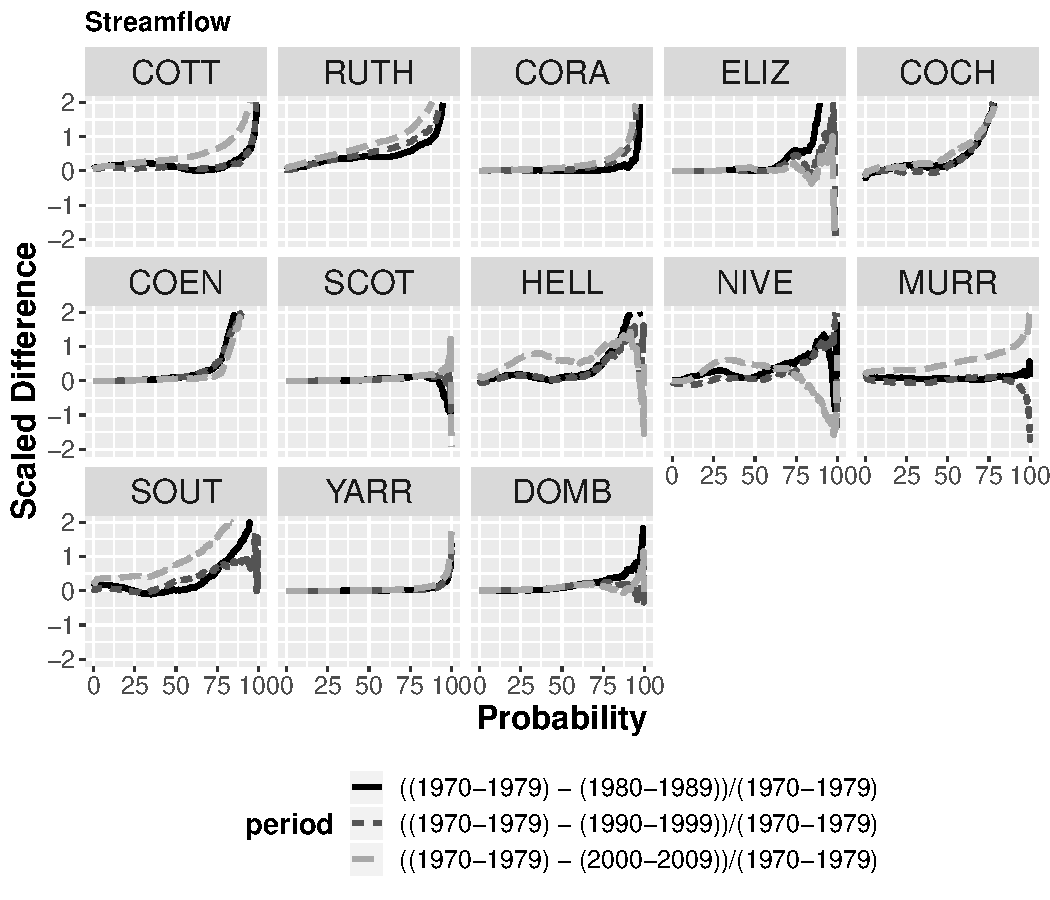
\includegraphics{4.FDC_Analysis_files/figure-latex/FDC_flow-1.pdf}
\caption{Difference in flow duration curves based on daily data split by
decade}
\end{figure}

\begin{Shaded}
\begin{Highlighting}[]
\CommentTok{# # publication quality}
\CommentTok{# tiff("../manuscript/Figure6_StreamflowFDCDifference.tif",}
\CommentTok{#      width=16*480, height=12*480,}
\CommentTok{#      res=600, compression="lzw")}
\CommentTok{# print(p)}
\CommentTok{# dev.off()}
\end{Highlighting}
\end{Shaded}

\subsection{daily rainfall data}\label{daily-rainfall-data}

\begin{Shaded}
\begin{Highlighting}[]
\CommentTok{# combine flow_zoo with flow_decade in a data.frame}
\NormalTok{rain_df <-}\StringTok{ }\KeywordTok{data.frame}\NormalTok{(}\DataTypeTok{decade=}\NormalTok{flow_decade,}
                         \KeywordTok{as.data.frame}\NormalTok{(rain_zoo))}
\CommentTok{# now calculate the rainfall duration curve for each catchment by decade}
\CommentTok{# tapply this across the columns and produce a list}
\CommentTok{# do this for each decade}
\CommentTok{# an empty list for the decades}
\NormalTok{FDCs <-}\StringTok{ }\KeywordTok{list}\NormalTok{()}
\NormalTok{for (i in }\DecValTok{1}\NormalTok{:}\DecValTok{4}\NormalTok{) \{}
  \NormalTok{FDCs[[i]] <-}\StringTok{ }\KeywordTok{apply}\NormalTok{(}\KeywordTok{subset}\NormalTok{(rain_df,}
      \KeywordTok{as.character}\NormalTok{(rain_df$decade)==}\KeywordTok{as.character}\NormalTok{(decades[i]))[,}\DecValTok{2}\NormalTok{:}\DecValTok{14}\NormalTok{],}
                      \DecValTok{2}\NormalTok{,FDC_gen)}
\NormalTok{\}}

\CommentTok{# DIFFERENCE BETWEEN WEEKLY FDCs DIVIDED BY 1970-1979 FDCs -> not log, ylim=c(-1,1) to prevent issues plotting when denominator 0 (gives -Inf) hence not all values shown}
\NormalTok{plot.list <-}\StringTok{ }\KeywordTok{vector}\NormalTok{(}\StringTok{"list"}\NormalTok{, }\DataTypeTok{length=}\DecValTok{13}\NormalTok{)}
\NormalTok{temp <-}\StringTok{ }\KeywordTok{list}\NormalTok{()}
\NormalTok{for (j in }\DecValTok{1}\NormalTok{:}\KeywordTok{length}\NormalTok{(periods)) \{}
  \NormalTok{for (i in }\KeywordTok{seq_along}\NormalTok{(Stations[,}\DecValTok{1}\NormalTok{])) \{}
    \NormalTok{temp[[i]] <-}\StringTok{ }\NormalTok{(FDCs[[}\DecValTok{1}\NormalTok{]][[i]]$flow -}\StringTok{ }\NormalTok{FDCs[[j}\DecValTok{+1}\NormalTok{]][[i]]$flow)/FDCs[[}\DecValTok{1}\NormalTok{]][[i]]$flow}
  \NormalTok{\}}
  \NormalTok{fdc <-}\StringTok{ }\KeywordTok{do.call}\NormalTok{(cbind,temp)}
  \KeywordTok{colnames}\NormalTok{(fdc) <-}\StringTok{ }\NormalTok{Stations[,}\DecValTok{1}\NormalTok{]}
  \NormalTok{plot.list[[j]] <-}\StringTok{ }\KeywordTok{melt}\NormalTok{(}\KeywordTok{data.frame}\NormalTok{(}\DataTypeTok{fdc =} \NormalTok{fdc, }
                                \DataTypeTok{period =} \KeywordTok{rep}\NormalTok{(periods[j],}\KeywordTok{nrow}\NormalTok{(fdc))),}
                                \DataTypeTok{id.vars=}\StringTok{"period"}\NormalTok{)}
\NormalTok{\}}
\CommentTok{# bring back together to a dataframe}
\NormalTok{plot_df_r <-}\StringTok{ }\KeywordTok{do.call}\NormalTok{(rbind,plot.list)}
\CommentTok{# add the probabilities}
\NormalTok{plot_df_r <-}\StringTok{ }\KeywordTok{cbind}\NormalTok{(plot_df_r,}\DataTypeTok{probs=}\KeywordTok{rep}\NormalTok{(FDCs[[}\DecValTok{1}\NormalTok{]][[}\DecValTok{1}\NormalTok{]]$probs,}\DecValTok{13}\NormalTok{*}\DecValTok{3}\NormalTok{))}
\KeywordTok{colnames}\NormalTok{(plot_df_r)[}\DecValTok{2}\NormalTok{] <-}\StringTok{ "station"}
\KeywordTok{levels}\NormalTok{(plot_df_r$station) <-}\StringTok{ }\NormalTok{Stations[,}\DecValTok{1}\NormalTok{]}

\CommentTok{# make a plot}
\NormalTok{p <-}\StringTok{ }\KeywordTok{ggplot}\NormalTok{(plot_df_r, }\KeywordTok{aes}\NormalTok{(}\DataTypeTok{x =} \NormalTok{probs, }\DataTypeTok{y =} \NormalTok{value)) +}
\StringTok{  }\KeywordTok{geom_line}\NormalTok{(}\KeywordTok{aes}\NormalTok{(}\DataTypeTok{linetype=}\NormalTok{period, }\DataTypeTok{colour=}\NormalTok{period),}\DataTypeTok{size=}\FloatTok{1.2}\NormalTok{) +}\StringTok{ }
\StringTok{  }\KeywordTok{facet_wrap}\NormalTok{(~}\StringTok{ }\NormalTok{station,}\DataTypeTok{ncol=}\DecValTok{5}\NormalTok{) +}\StringTok{ }\KeywordTok{ylim}\NormalTok{(}\KeywordTok{c}\NormalTok{(-}\DecValTok{2}\NormalTok{,}\DecValTok{2}\NormalTok{)) +}
\StringTok{  }\KeywordTok{theme}\NormalTok{(}\DataTypeTok{legend.position=}\StringTok{"bottom"}\NormalTok{) +}
\StringTok{  }\KeywordTok{guides}\NormalTok{(}\DataTypeTok{col =} \KeywordTok{guide_legend}\NormalTok{(}\DataTypeTok{nrow =} \DecValTok{3}\NormalTok{))}
\NormalTok{p <-}\StringTok{ }\NormalTok{p +}\StringTok{ }\KeywordTok{ggtitle}\NormalTok{(}\StringTok{"Rainfall"}\NormalTok{) +}
\StringTok{  }\KeywordTok{theme}\NormalTok{(}\DataTypeTok{plot.title =} \KeywordTok{element_text}\NormalTok{(}\DataTypeTok{lineheight=}\NormalTok{.}\DecValTok{8}\NormalTok{, }\DataTypeTok{face=}\StringTok{"bold"}\NormalTok{))+}
\StringTok{  }\KeywordTok{xlab}\NormalTok{(}\StringTok{"Probability"}\NormalTok{) +}
\StringTok{  }\KeywordTok{theme}\NormalTok{(}\DataTypeTok{axis.title.x =} \KeywordTok{element_text}\NormalTok{(}\DataTypeTok{face=}\StringTok{"bold"}\NormalTok{,  }\DataTypeTok{size=}\DecValTok{16}\NormalTok{),}
        \DataTypeTok{axis.text.x  =} \KeywordTok{element_text}\NormalTok{(}\DataTypeTok{size=}\DecValTok{12}\NormalTok{)) +}
\StringTok{  }\KeywordTok{ylab}\NormalTok{(}\StringTok{"Scaled Difference"}\NormalTok{) +}
\StringTok{  }\KeywordTok{theme}\NormalTok{(}\DataTypeTok{axis.title.y =} \KeywordTok{element_text}\NormalTok{(}\DataTypeTok{face=}\StringTok{"bold"}\NormalTok{,  }\DataTypeTok{size=}\DecValTok{16}\NormalTok{),}
        \DataTypeTok{axis.text.y  =} \KeywordTok{element_text}\NormalTok{(}\DataTypeTok{size=}\DecValTok{12}\NormalTok{)) +}
\StringTok{ }\KeywordTok{scale_colour_manual}\NormalTok{(}\DataTypeTok{values=}\KeywordTok{c}\NormalTok{(}\StringTok{"black"}\NormalTok{, }\StringTok{"gray33"}\NormalTok{, }\StringTok{"gray66"}\NormalTok{)) +}
\StringTok{  }\KeywordTok{theme}\NormalTok{(}\DataTypeTok{legend.text =} \KeywordTok{element_text}\NormalTok{( }\DataTypeTok{size =} \DecValTok{12}\NormalTok{))+}
\StringTok{  }\KeywordTok{theme}\NormalTok{(}\DataTypeTok{legend.title =} \KeywordTok{element_text}\NormalTok{(}\DataTypeTok{size=}\DecValTok{14}\NormalTok{, }\DataTypeTok{face=}\StringTok{"bold"}\NormalTok{)) +}
\StringTok{  }\KeywordTok{theme}\NormalTok{(}\DataTypeTok{strip.text.x =} \KeywordTok{element_text}\NormalTok{(}\DataTypeTok{size=}\DecValTok{16}\NormalTok{))}
\KeywordTok{print}\NormalTok{(p)}
\end{Highlighting}
\end{Shaded}

\begin{verbatim}
## Warning: Removed 1887 rows containing missing values (geom_path).
\end{verbatim}

\begin{figure}[htbp]
\centering
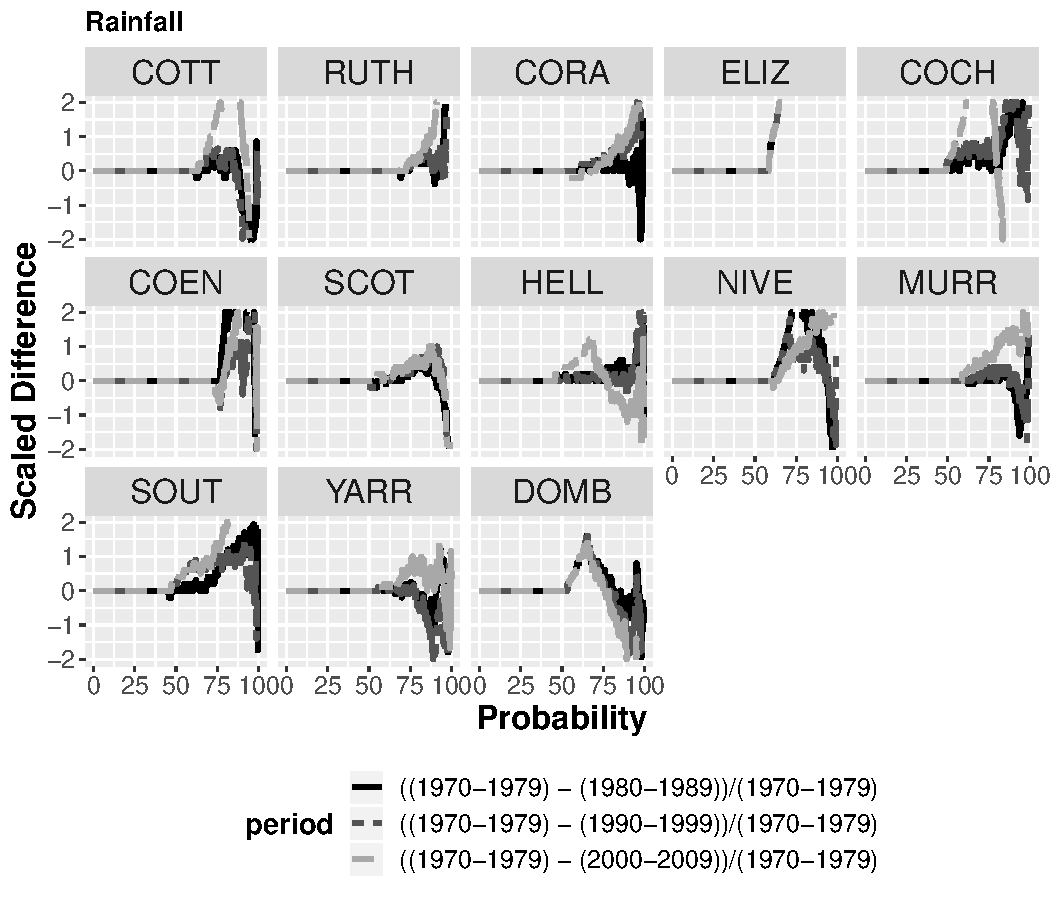
\includegraphics{4.FDC_Analysis_files/figure-latex/FDC_rain-1.pdf}
\caption{Difference in rainfal duration curves based on daily data split
by decade}
\end{figure}

\begin{Shaded}
\begin{Highlighting}[]
\CommentTok{# publication quality}
\CommentTok{# tiff("../manuscript/Figure7_RainfallFDCDifference.tif",}
\CommentTok{#      width=16*480, height=12*480,}
\CommentTok{#      res=600, compression="lzw")}
\CommentTok{# print(p)}
\CommentTok{# dev.off()}
\end{Highlighting}
\end{Shaded}

\subsection{daily gridded rainfall}\label{daily-gridded-rainfall}

\begin{Shaded}
\begin{Highlighting}[]
\CommentTok{# gridded rainfall}
\NormalTok{grrain_df <-}\StringTok{ }\KeywordTok{data.frame}\NormalTok{(}\DataTypeTok{decade=}\KeywordTok{rep}\NormalTok{(flow_decade,}\DecValTok{13}\NormalTok{),}
                         \KeywordTok{as.data.frame}\NormalTok{(GridRainAllDataout[,}\DecValTok{1}\NormalTok{:}\DecValTok{2}\NormalTok{]))}
\CommentTok{# now calculate the rainfall duration curve for each catchment by decade}
\CommentTok{# tapply this across the columns and produce a list}
\CommentTok{# do this for each decade}
\CommentTok{# an empty list for the decades}
\NormalTok{FDCs <-}\StringTok{ }\KeywordTok{list}\NormalTok{()}
\NormalTok{for (i in }\DecValTok{1}\NormalTok{:}\DecValTok{4}\NormalTok{) \{}
  \NormalTok{temp <-}\StringTok{ }\KeywordTok{subset}\NormalTok{(grrain_df,}
                        \KeywordTok{as.character}\NormalTok{(grrain_df$decade)==}\StringTok{  }
\StringTok{                        }\KeywordTok{as.character}\NormalTok{(decades[i]))}
  \NormalTok{FDCs[[i]] <-}\StringTok{ }\KeywordTok{tapply}\NormalTok{(temp[,}\StringTok{"gridRain"}\NormalTok{],}
                      \KeywordTok{list}\NormalTok{(}\DataTypeTok{Station=}\NormalTok{temp$Station),FDC_gen)}
\NormalTok{\}}

\CommentTok{# plotting}
\NormalTok{plot.list <-}\StringTok{ }\KeywordTok{vector}\NormalTok{(}\StringTok{"list"}\NormalTok{, }\DataTypeTok{length=}\DecValTok{13}\NormalTok{)}
\NormalTok{temp <-}\StringTok{ }\KeywordTok{list}\NormalTok{()}
\NormalTok{for (j in }\DecValTok{1}\NormalTok{:}\KeywordTok{length}\NormalTok{(periods)) \{}
  \NormalTok{for (i in }\KeywordTok{seq_along}\NormalTok{(Stations[,}\DecValTok{1}\NormalTok{])) \{}
    \NormalTok{temp[[i]] <-}\StringTok{ }\NormalTok{(FDCs[[}\DecValTok{1}\NormalTok{]][[i]]$flow -}\StringTok{ }\NormalTok{FDCs[[j}\DecValTok{+1}\NormalTok{]][[i]]$flow)/FDCs[[}\DecValTok{1}\NormalTok{]][[i]]$flow}
  \NormalTok{\}}
  \NormalTok{fdc <-}\StringTok{ }\KeywordTok{do.call}\NormalTok{(cbind,temp)}
  \KeywordTok{colnames}\NormalTok{(fdc) <-}\StringTok{ }\NormalTok{Stations[,}\DecValTok{1}\NormalTok{]}
  \NormalTok{plot.list[[j]] <-}\StringTok{ }\KeywordTok{melt}\NormalTok{(}\KeywordTok{data.frame}\NormalTok{(}\DataTypeTok{fdc =} \NormalTok{fdc, }
                                \DataTypeTok{period =} \KeywordTok{rep}\NormalTok{(periods[j],}\KeywordTok{nrow}\NormalTok{(fdc))),}
                                \DataTypeTok{id.vars=}\StringTok{"period"}\NormalTok{)}
\NormalTok{\}}
\CommentTok{# bring back together to a dataframe}
\NormalTok{plot_df_r <-}\StringTok{ }\KeywordTok{do.call}\NormalTok{(rbind,plot.list)}
\CommentTok{# add the probabilities}
\NormalTok{plot_df_r <-}\StringTok{ }\KeywordTok{cbind}\NormalTok{(plot_df_r,}\DataTypeTok{probs=}\KeywordTok{rep}\NormalTok{(FDCs[[}\DecValTok{1}\NormalTok{]][[}\DecValTok{1}\NormalTok{]]$probs,}\DecValTok{13}\NormalTok{*}\DecValTok{3}\NormalTok{))}
\KeywordTok{colnames}\NormalTok{(plot_df_r)[}\DecValTok{2}\NormalTok{] <-}\StringTok{ "station"}
\KeywordTok{levels}\NormalTok{(plot_df_r$station) <-}\StringTok{ }\NormalTok{Stations[,}\DecValTok{1}\NormalTok{]}

\CommentTok{# make a plot}
\NormalTok{p <-}\StringTok{ }\KeywordTok{ggplot}\NormalTok{(plot_df_r, }\KeywordTok{aes}\NormalTok{(}\DataTypeTok{x =} \NormalTok{probs, }\DataTypeTok{y =} \NormalTok{value)) +}
\StringTok{  }\KeywordTok{geom_line}\NormalTok{(}\KeywordTok{aes}\NormalTok{(}\DataTypeTok{linetype=}\NormalTok{period, }\DataTypeTok{colour=}\NormalTok{period),}\DataTypeTok{size=}\FloatTok{1.2}\NormalTok{) +}\StringTok{ }
\StringTok{  }\KeywordTok{facet_wrap}\NormalTok{(~}\StringTok{ }\NormalTok{station,}\DataTypeTok{ncol=}\DecValTok{5}\NormalTok{) +}\StringTok{ }\KeywordTok{ylim}\NormalTok{(}\KeywordTok{c}\NormalTok{(-}\DecValTok{2}\NormalTok{,}\DecValTok{2}\NormalTok{)) +}
\StringTok{  }\KeywordTok{theme}\NormalTok{(}\DataTypeTok{legend.position=}\StringTok{"bottom"}\NormalTok{) +}
\StringTok{  }\KeywordTok{guides}\NormalTok{(}\DataTypeTok{col =} \KeywordTok{guide_legend}\NormalTok{(}\DataTypeTok{nrow =} \DecValTok{3}\NormalTok{))}
\NormalTok{p <-}\StringTok{ }\NormalTok{p +}\StringTok{ }\KeywordTok{ggtitle}\NormalTok{(}\StringTok{"gridded Rainfall"}\NormalTok{) +}
\StringTok{  }\KeywordTok{theme}\NormalTok{(}\DataTypeTok{plot.title =} \KeywordTok{element_text}\NormalTok{(}\DataTypeTok{lineheight=}\NormalTok{.}\DecValTok{8}\NormalTok{, }\DataTypeTok{face=}\StringTok{"bold"}\NormalTok{))+}
\StringTok{  }\KeywordTok{xlab}\NormalTok{(}\StringTok{"Probability"}\NormalTok{) +}
\StringTok{  }\KeywordTok{theme}\NormalTok{(}\DataTypeTok{axis.title.x =} \KeywordTok{element_text}\NormalTok{(}\DataTypeTok{face=}\StringTok{"bold"}\NormalTok{,  }\DataTypeTok{size=}\DecValTok{16}\NormalTok{),}
        \DataTypeTok{axis.text.x  =} \KeywordTok{element_text}\NormalTok{(}\DataTypeTok{size=}\DecValTok{12}\NormalTok{)) +}
\StringTok{  }\KeywordTok{ylab}\NormalTok{(}\StringTok{"Scaled Difference"}\NormalTok{) +}
\StringTok{  }\KeywordTok{theme}\NormalTok{(}\DataTypeTok{axis.title.y =} \KeywordTok{element_text}\NormalTok{(}\DataTypeTok{face=}\StringTok{"bold"}\NormalTok{,  }\DataTypeTok{size=}\DecValTok{16}\NormalTok{),}
        \DataTypeTok{axis.text.y  =} \KeywordTok{element_text}\NormalTok{(}\DataTypeTok{size=}\DecValTok{12}\NormalTok{)) +}
\StringTok{ }\KeywordTok{scale_colour_manual}\NormalTok{(}\DataTypeTok{values=}\KeywordTok{c}\NormalTok{(}\StringTok{"black"}\NormalTok{, }\StringTok{"gray33"}\NormalTok{, }\StringTok{"gray66"}\NormalTok{)) +}
\StringTok{  }\KeywordTok{theme}\NormalTok{(}\DataTypeTok{legend.text =} \KeywordTok{element_text}\NormalTok{( }\DataTypeTok{size =} \DecValTok{12}\NormalTok{))+}
\StringTok{  }\KeywordTok{theme}\NormalTok{(}\DataTypeTok{legend.title =} \KeywordTok{element_text}\NormalTok{(}\DataTypeTok{size=}\DecValTok{14}\NormalTok{, }\DataTypeTok{face=}\StringTok{"bold"}\NormalTok{)) +}
\StringTok{  }\KeywordTok{theme}\NormalTok{(}\DataTypeTok{strip.text.x =} \KeywordTok{element_text}\NormalTok{(}\DataTypeTok{size=}\DecValTok{16}\NormalTok{))}
\KeywordTok{print}\NormalTok{(p)}
\end{Highlighting}
\end{Shaded}

\begin{verbatim}
## Warning: Removed 39 rows containing missing values (geom_path).
\end{verbatim}

\begin{figure}[htbp]
\centering
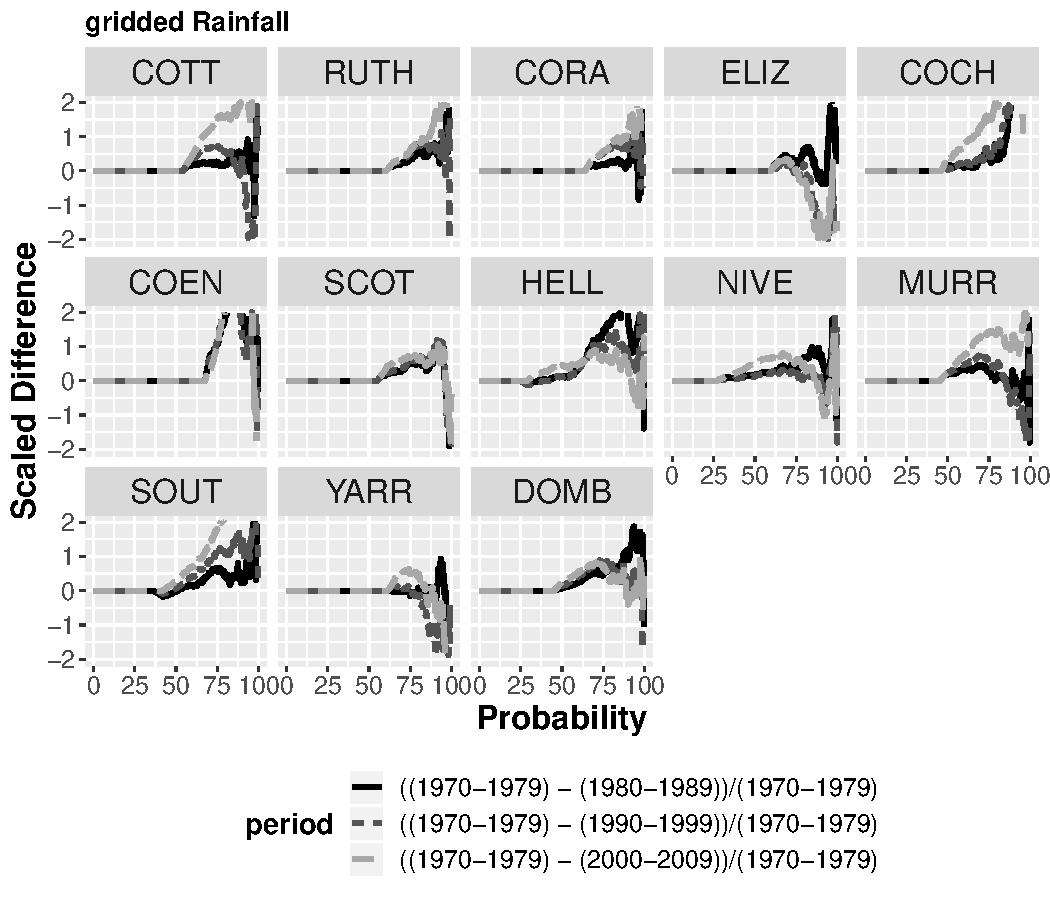
\includegraphics{4.FDC_Analysis_files/figure-latex/FDC_gridRain-1.pdf}
\caption{Difference in gridded rainfal duration curves based on daily
gridded data split by decade}
\end{figure}


\end{document}
